\chapter{Background}

Malware is a software program intended to do pernicious activities on a client`s computer with the proposition of removing data and misusing assets without his assent. Viruses and worms are the best known types of malware on account of the way in which they spread, instead of their behavior. Malware is now and then utilized widely against government or corporate websites to gather protected data or to disturb their operations by large. Also, malware is regularly utilized against people to steal data, for example, personal identification numbers or bank or credit card details and passwords. As per a survey on data breaches led by Verizon in 2014 \cite{bib9}, Citadel is the preferred banking malware among attackers for stealing individual information. And for stealing money from bank accounts, Zeus is the favorite banking malware.

Figure 1 shows how the malware is swiftly growing in volume day-by-day. In Figure 1, the x-axis specifies the year and the y-axis indicates the number of malware samples generated in the specified year on the x-axis.

\begin{figure}
    \centering    
    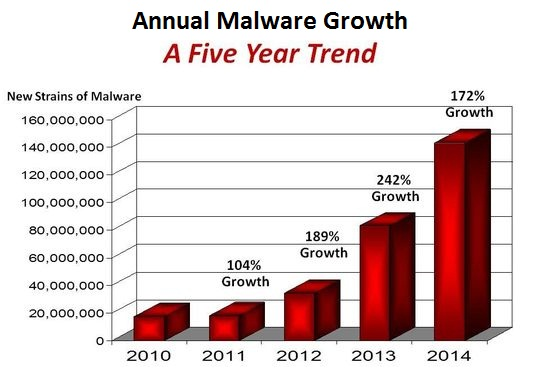
\includegraphics[width=8.4cm, height=6cm]{malware-growth-chart.jpg}
    \caption[Annual Malware Growth]{Annual Malware Growth \cite{bib10}}
\end{figure}
Virus writers are aware that signature-based detection with heuristic analysis can be the basis of modern malware detection techniques. So, virus developers have created numerous procedures and techniques to evade signature-based detection. In January 2015, AV-TEST`s CEO said, "Many of the new malware samples are just variants of existing viruses. They have been modified so that they are no longer detected and thus, AV signature updates are required" \cite{bib10}. Some of the noteworthy techniques used by virus writers to evade signature detection are encryption, polymorphism and metamorphism.

\section{Encrypted Malware} 

The Cascade virus, which initially appeared in late 1986, was the first malware that used encryption to scramble its contents \cite{bib11}. The Cascade virus is comprised of two parts. The first part is a decryptor and the second part is encrypted malware code. The reason for encryption is to conceal the malware signature, so as to evade signature identification. Later, this technique was adopted by almost every encrypted malware.  For the most part, virus writers use extremely simple and weak encryption methods, for example, a repeated XOR with a fixed bit pattern. Cascade malware also used XOR operation as encryption routine because of its symmetrical and reversible feature. In the event that the encryption key of malware was changed after every infection, the encrypted body signature also gets changed. If in case the same decryptor was used, signature detection can make use of the decryptor code`s signature to detect the malware.
\begin{figure}
    \centering    
    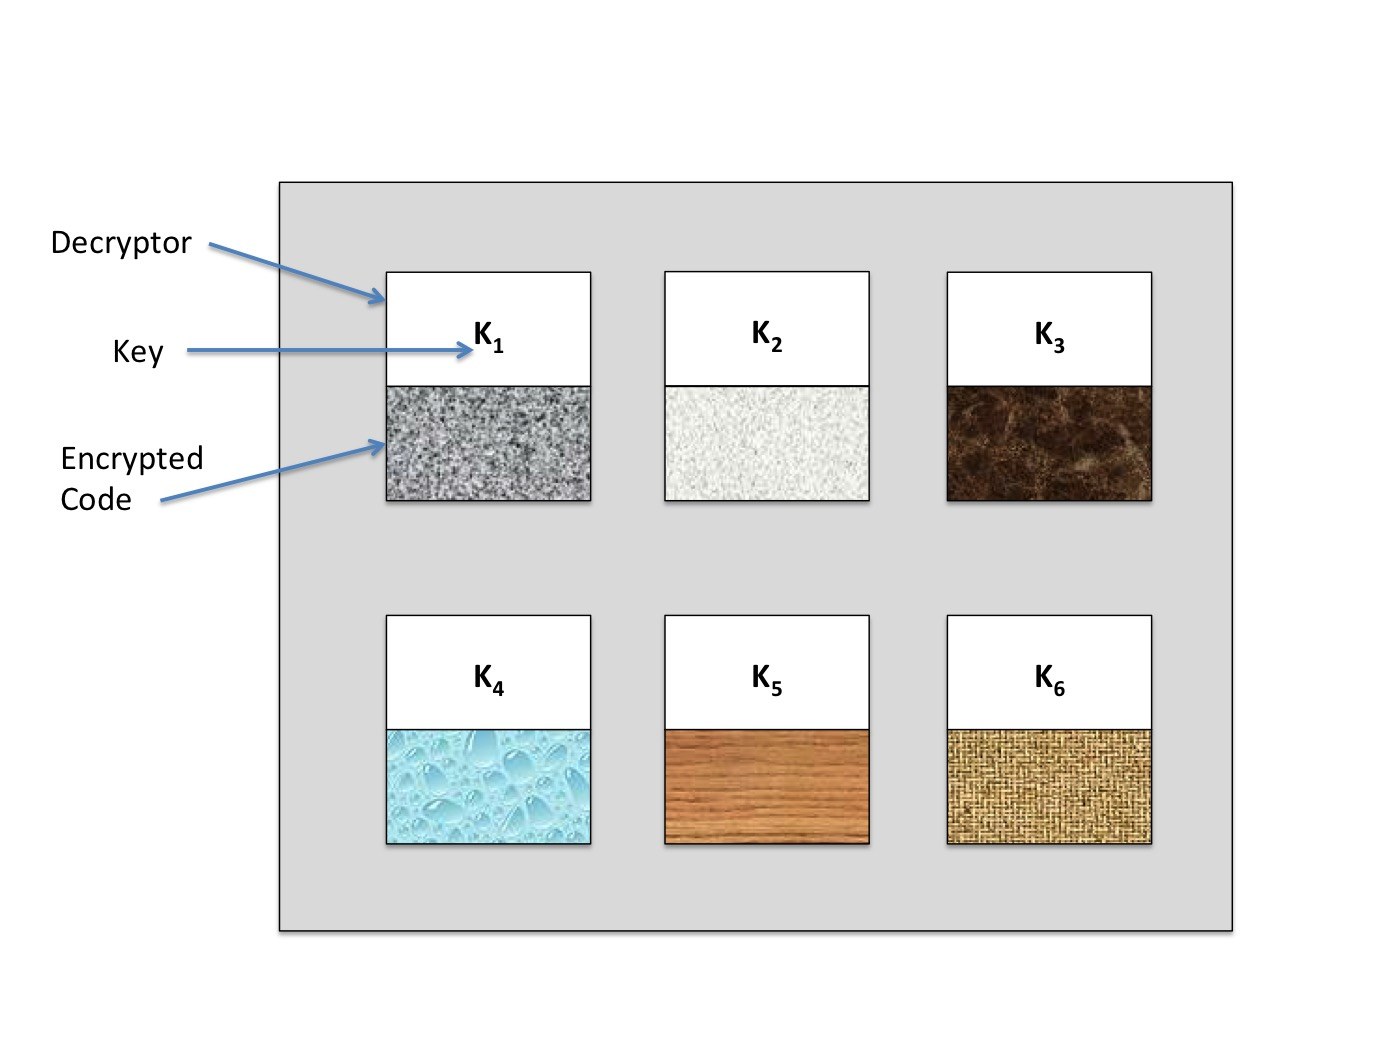
\includegraphics[width=8cm, height=6cm]{encryptedvirus.jpg}
    \caption[Encrypted Malware Replication]{An Encrypting malware spreads without changing decryptor but the key within decryptor varies from infection to infection. As the key value changes, the encrypted virus body also changes \cite{bib14}.}
\end{figure}
\section{Polymorphic Malware} 

Similar to an encrypted malware, polymorphic malware incorporates an encrypted virus code and a decryptor. Additionally in a polymorphic virus, the decryptor is morphed. During polymorphic malware propogation, not only is the virus code encrypted, but the decryptor also varies from infection to infection. As there is no fixed signature or no fixed decryptor to scan for, no two infections look alike to be exploited by the antivirus program for detection purpose \cite{bib14}. Polymorphic virus uses code obfuscation techniques, for example, including junk codes or substitution of instructions, to mutate its decryptor \cite{bib18}.
Several techniques are utilized to decrypt the polymorphic virus, such as, cryptanalysis (also called x-ray), emulation and dedicated decryption routines \cite{bib21}.

\begin{figure}
  \centering
\begin{lstlisting}[language=myasm]
MOV A,R$1$         MOV A,R$1$        MOV A,R$1$         MOV A,R$1$         MOV A,R$1$
ADD B,R$1$         NOP            ADD #0,R$1$        OR R$1$,R$1$          TST R$1$
ADD C,R$1$         ADD B,R$1$        ADD B,R$1$         ADD B,R$1$         ADD C,R$1$
SUB #4,R$1$        NOP            OR R$1$,R$1$          MOV R$1$,R$5$         MOV R$1$,R$5$
MOV R$1$,X         ADD C,R$1$        ADD C,R$1$         ADD C,R$1$         ADD B,R$1$
                NOP            SHL #0,R$1$        SHL R$1$,0         CMP R$2$,R$5$
                SUB #4,R$1$       SUB #4,R$1$        SUB #4,R$1$        SUB #4,R$1$
                NOP            JMP .+1         ADD R$5$,R$5$         JMP .+1
                MOV R$1$,X        MOV R$1$,X         MOV R$1$,X         MOV R$1$,X
                                               MOV R$5$,Y         MOV R$5$,Y
(a)             (b)             (c)             (d)             (e)


\end{lstlisting}
    \caption[Examples of a polymorphic virus.]{Examples of a polymorphic virus utilizing code obfuscation techniques. All of the Figure~\ref{fig:polyvirus} snippets perform the same operation, i.e.,  $X = (A + B + C - 4)$. For instance, the program snippet of Figure~\ref{fig:polyvirus} (c) is functionally the same as Figure~\ref{fig:polyvirus} (a) in light of the fact that instructions like adding 0 to a register, ORing R1 with itself, shifting R1 left 0 bits, and jumping to the next instruction all do nothing \cite{bib19}.}
    \label{fig:polyvirus}
\end{figure}

    
The first polymorphic malware, 1260, was developed by Mark Washburn in 1990 \cite{bib15}. And the first widespread polymorphic infection was caused by Tequila and Maltese Amoeba virus, in 1991 \cite{bib14}.

\section{Metamorphic Malware} 

Virus writers took the next step and developed an advanced variant of polymorphic malware, known as metamorphic malware. Generally, before infection, polymorphic malware encrypt the virus code and morph the decryptor, while metamorphic malware morph the whole virus code. According to Igor Muttik, "Metamorphics are bodypolymorphics", since polymorphism is applied to the entire virus body \cite{bib22}. Metamorphic viruses utilizes several code morphing techniques that constitute instruction reordering, data reordering, subroutine inlining, subroutine outlining, register renaming, instruction substitution and dead code insertion \cite{bib23}. Figure~\ref{fig:aimalware} illustrates the metamorphic malware with different signatures.

\begin{figure}
  \centering
      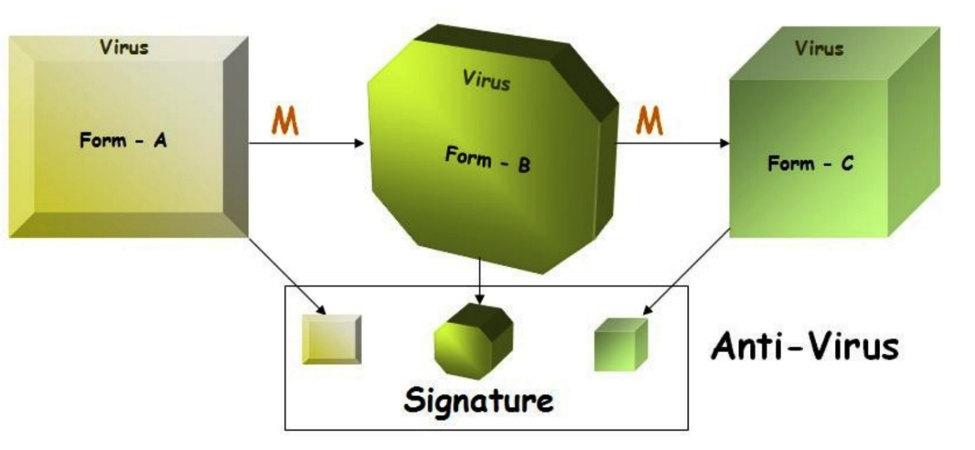
\includegraphics[width=9cm, height=4.5cm]{aimalwarepic.png}
    \caption[Metamorphic malware with different signatures]{Metamorphic malware with different signatures \cite{bib20}.}
    \label{fig:aimalware}
\end{figure}

\subsection{Register renaming} 

In December 1998, a metamorphic malware named Win95/Regswap was developed by Vecna \cite{bib22}. Regswap used register renaming technique to morph the virus code. In this technique, instructions gets modified to use different registers. As just the register operands gets altered that too in some part of the code instead of whole code, so the complexity of final modified code wouldn`t be high. Figure~\ref{fig:regswap} depicts how the register renaming technique transforms the code.

\begin{figure}
  \centering
      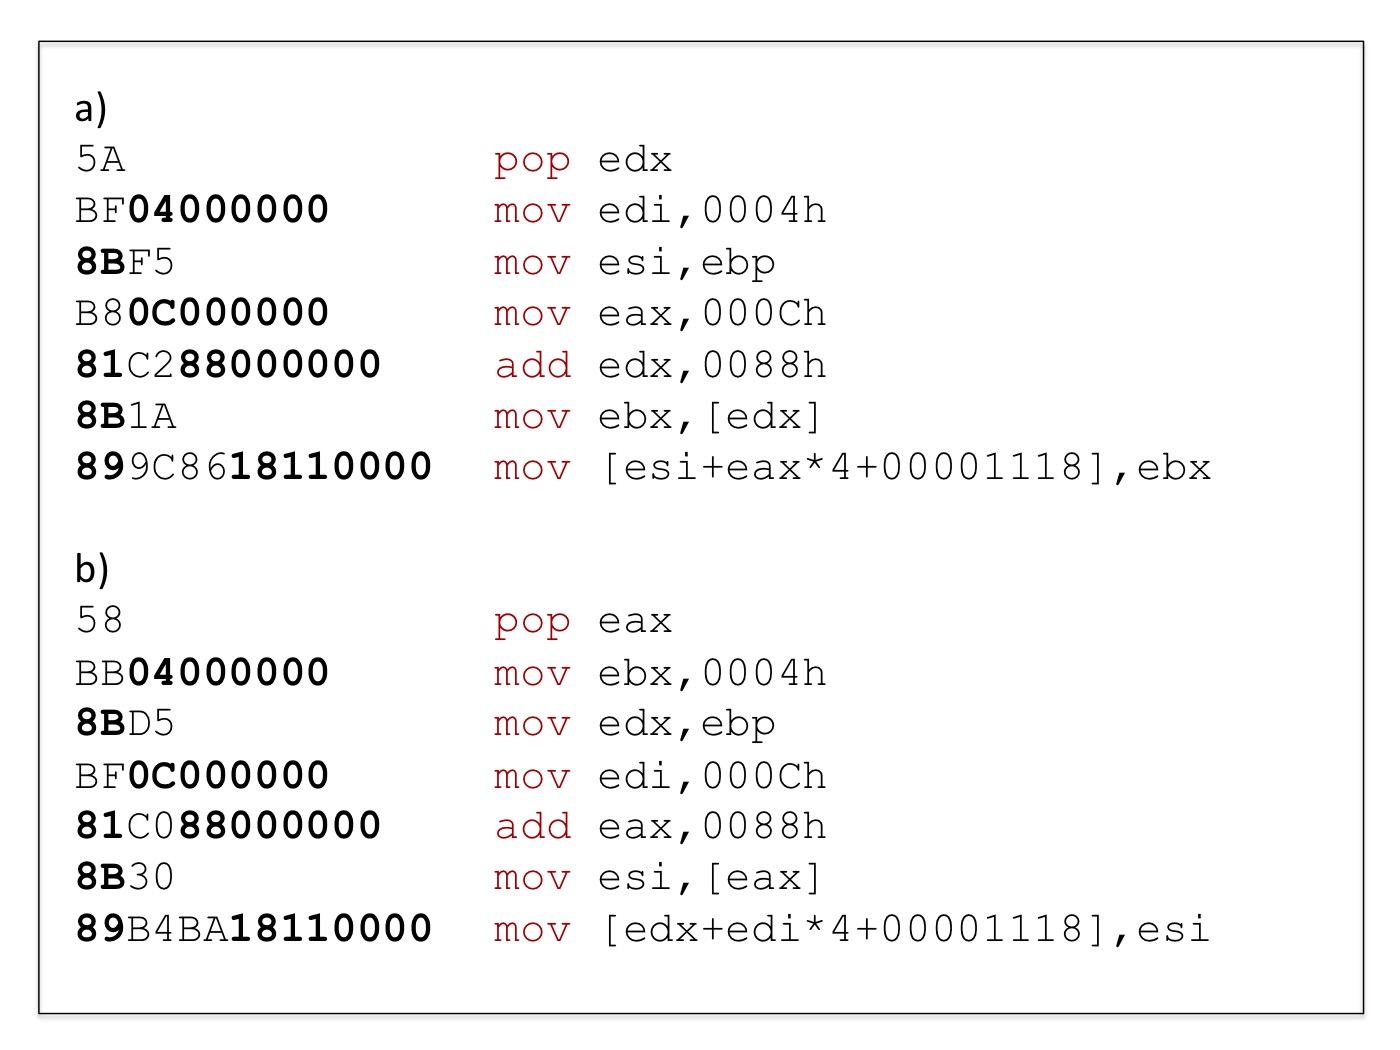
\includegraphics[width=12.9cm, height=9cm]{regswap.jpg}
    \caption[Register Renaming Example]{code snippet extracted from two different versions of RegSwap \cite{bib22}.}
    \label{fig:regswap}
\end{figure}

The bold areas in figure~\ref{fig:regswap} illustrates the similarities of the two different code versions. Thus, a wildcard string, such as $5? B?$, could be useful to detect the malware code \cite{bib22}. 

\subsection{Dead code insertion} 

Dead code can be a single instruction or a block of instructions, for example, adding NOPs \cite{bib23}, adding 0 to a register, moving between same registers, ORing register with itself, shifting register left 0 bits, jumping to next instruction, incrementing a register immediately followed by decrementing the same register by same value. Inserting dead code or do-nothing instructions is the easiest approach to morph the virus code without modifying its functionality \cite{bib23}. 
The Win32/Evol virus, which was found around July 2000 \cite{bib24}, used dead code insertion to obfuscate the signature of a code as illustrated in Figure~\ref{fig:deadcode}. 

\begin{figure}
  \centering
  \begin{lstlisting}[language=myasm]
C$7060$F$000055$				MOV [esi], $5500000$Fh
C$746048$BEC$5151$		MOV [esi+0004], $5151$EC$8$Bh
BF$0$F$00055$					MOV edi, $5500000$Fh
$893$E 						MOV [esi], edi
$5$F 						POP edi						; garbage
52 					PUSH edx						; garbage
B$640$ 						MOV dh, 40 					; garbage
BA$8$BEC$5151$ 				MOV edx, $5151$EC$8$Bh
53 					PUSH ebx						; garbage
$8$BDA					MOV ebx, edx
$895$E$04$						MOV [esi+0004], ebx  
\end{lstlisting}
    \caption[Example of code metamorphosis of Evol virus ]{Example of code metamorphosis of Evol virus with Dead code insertion \cite{bib23}.}
    \label{fig:deadcode}
\end{figure}

\subsection{Subroutine permutation} 

Code may contain several subroutines (or) functions and changing the order of this subroutines may not impact the execution of code. Subroutine permutation approach makes use of this advantage i.e., altering the order of subroutines, to change its internal structure without modifying the functionality of code. A code with $n$ different subroutines can generate $n!$ different permutations of subroutines, thus large number of versions of the same code can be generated \cite{bib4}.

\begin{figure}
  \centering
      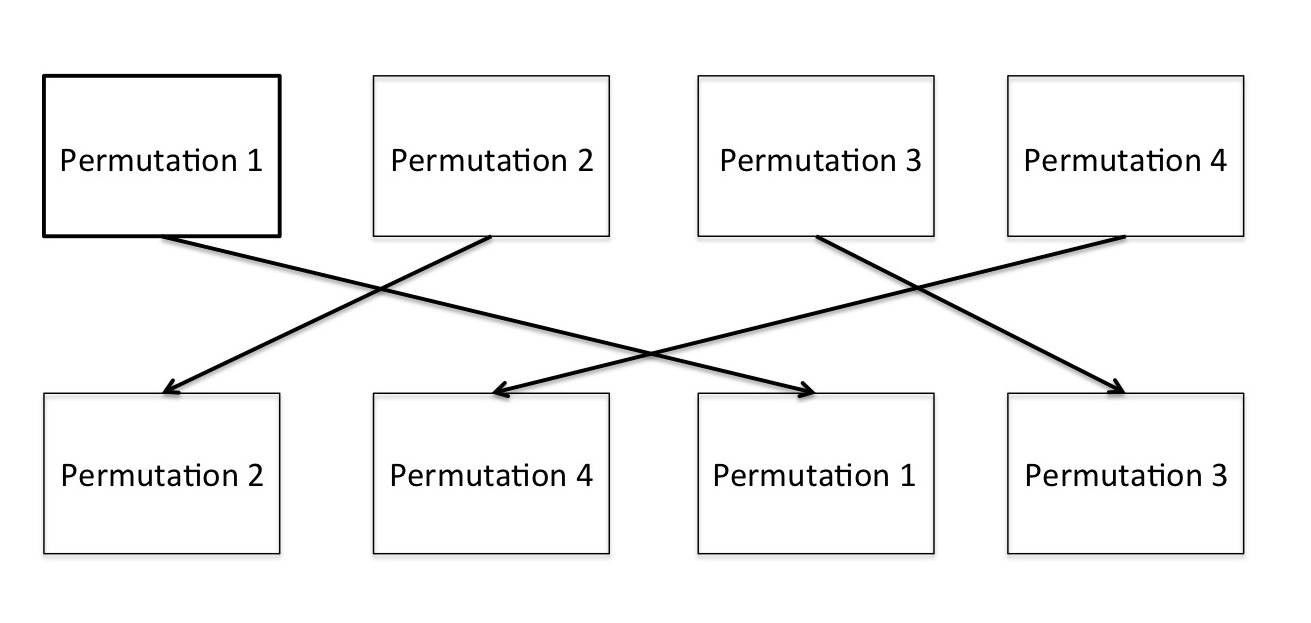
\includegraphics[width=12cm, height=6cm]{subpermutation.jpg}
    \caption[Example of subroutines permutation]{Example of subroutines permutation \cite{bib23}.}
    \label{fig:subpermutation}
\end{figure}

\subsection{Equivalent code substitution} 
Different variants of code can be generated by replacing instruction or block of instructions with an equivalent code. In assembly language there are numerous semantically equivalent instructions, for instance, `INC ecx' is same as `ADD ecx, 1', `XOR R1, R1' is same as `MOV R1, 0' \cite{bib25}.

\subsection{Transposition} 
Morphed copies of virus code can also be created by changing the order of instructions in the code provided that there is no dependency among instructions, so this approach is also known as instruction permutation \cite{bib23}. For instance, the code in figure~\ref{fig:beforetrans} can be transformed to figure~\ref{fig:aftertrans}, as the declaration order of variables doesn`t affect the arithmetic calculation \cite{bib4}. 

\begin{figure}
  \centering
  \begin{lstlisting}[language=Java]
  int a=5;
  int b=2;
  int c=a+b;
\end{lstlisting}
    \caption[Sample Java code]{Sample Java code \cite{bib4}.}
    \label{fig:beforetrans}
\end{figure}

\begin{figure}
  \centering
  \begin{lstlisting}[language=Java]
  int b=2;
  int a=5;
  int c=a+b;
\end{lstlisting}
    \caption[Sample Java code after applying Transposition]{Sample Java code after swapping instructions  \cite{bib4}.}
    \label{fig:aftertrans}
\end{figure}

\subsection{Changing control flow} 
The next code obfuscation method involves insertion of a conditional or unconditional branch instruction after a block of instructions. Further, instruction blocks referenced by this branching instructions can be permuted to change the control flow \cite{bib23}. Zperm malware used this approach to change the internal structure of a code \cite{bib25}. Figure ~\ref{fig:changecntflow} is an example of changing control flow.

\begin{figure}
  \centering
  \begin{lstlisting}[language=myasm]
;Original Program 
instruction 1   ; entry point
instruction 2
instruction 3
instruction 4
instruction 5
\end{lstlisting}

\begin{lstlisting}[language=myasm]
;Modified Program
instruction 2
jump 3
instruction 4
jump 5
instruction 1   ; entry point
jump 2
instruction 3
jump 4
instruction 5
\end{lstlisting}

    \caption[Example of changing control flow]{Example of changing control flow \cite{bib25}.}
    \label{fig:changecntflow}
\end{figure}

\subsection{Subroutine inlining and outlining} 
In subroutine inlining procedure, subroutine/function call replaces its code \cite{bib23}. Figure ~\ref{fig:subroutineinline} illustrates the concept of Subroutine inlining. 

\begin{figure}
  \centering
  \begin{lstlisting}[language=myasm]
	/* some instrictions */				/* some instrictions */ 
	call S1									mov eax, ebx
	call S2									add eax, 12h
	/* some instrictions */				push eax
	S1: 										mul ecx
	 mov eax, ebx							mov edx, eax
	 add eax, 12h							/* some instrictions */
	 push eax					
	 ret						
	S2:							
	 mul ecx
	 mov edx, eax
	 ret
(a) before transformation			(b) after transformation
\end{lstlisting}


    \caption[Subroutine inlining example]{Subroutine inlining example \cite{bib25}.}
    \label{fig:subroutineinline}
\end{figure}

On the other hand, code outlining changes a block of instructions into subroutine (or function) and a subroutine call will be included for the newly created subroutine. Figure ~\ref{fig:subroutineoutline} illustrates how the code outlining approach works.
\begin{figure}
  \centering
  \begin{lstlisting}[language=myasm]
	/* some instrictions */					/* some instrictions */
	mov  eax, ebx								mov  eax, ebx
	add  eax, 12h								call S1
	push eax										mov  edx, eax
	mul  ecx										/* some instrictions */
	mov  edx, eax								S1: 
	/* some instrictions */ 				 push eax
										 	 	 	 add  eax, 12h
										 	 	 	 mul  ecx
										 	 	 	 ret
(a) before transformation				(b) after transformation
\end{lstlisting}


    \caption[Subroutine outlining example]{Subroutine outlining example \cite{bib25}.}
    \label{fig:subroutineoutline}
\end{figure}

\section{Transcriptase} \label{transcriptasesection}

Transcriptase is a metamorphic virus implemented in JavaScript. Whenever Transcriptase is executed, a morphed version of the malware virus gets prepended to all the JavaScript files in the folder \cite{bib4}. The infected JavaScript file will become the variant of Transcriptase. By this way Transcriptase propagates and infects the benign JavaScript files.
  
The metamorphic engine attached to Transcriptase is a self-hosted compiler, which contains its own meta-language source-code. Transcriptase obtains information of its code from meta-language and changes its internal structure. 

The format of every line of the meta-code looks like \cite{bib26}:

\begin{lstlisting}[frame=none,numbers=none]
(Identifier|Restrictions)instruction
\end{lstlisting}
For instance, below are sample meta-instructions:

\begin{lstlisting}[frame=none,numbers=none,language=JavaScript]
(200|)var b=0
(300|200)c+1(b)
\end{lstlisting}

An Identifier and Restrictions are used by the Permutation function to do code obfuscation. The identifier is unique for every instruction in the entire code and restrictions specify the instructions on which the corresponding instruction is depending. The "instruction" contains the details used to create an actual code. 

The compiler creates the new malicious JavaScript code with three steps:

\begin{enumerate}
  \item Permutation and Variable/Function-Name randomization
  \item Code Creation
  \item Variable/Function insertion
\end{enumerate}

\subsection{Permutator}

In this phase, the compiler parses through every meta-language instruction, scope by scope (global scope for global instructions and sub-scope for if/for/while/functions) and retrieves the identifiers and restrictions details for each meta-instruction. Later these identifier and restriction details are used by the compiler to perform the permutation of code.

If the restriction details are empty for all the meta-language instructions, then it specifies that all the instructions in the code do not have any dependency instructions. So, the entire code can be permuted in all the possible combinations. For instance, if there are $n$ lines of code, then the permutator can create $n!$ variations of the original code. 

For instance, consider the code specified in Figure~\ref{fig:permutator} \cite{bib4}. It contains restriction details for some of the meta-instructions, which means that those instructions have dependencies on other instructions. So all the combinations of the code cannot produce the correct behaviour. 


\begin{figure}
  \centering
  \begin{lstlisting}[language=JavaScript]
	(100|)var a=5
	(200|)var b=-1
	(300|)var x=8
	(400|200)c+1(b)	// instruction c+1(b) means increment b by 1: i.e. b++
	(500|400,100)c+n(b,a) // instruction c+n(b,a) means increment b by a: i.e. b+=a
	(600|500)xWScript.Echo(x)
\end{lstlisting}

    \caption[Meta-language instructions example]{Meta-language instructions example \cite{bib4}.}
    \label{fig:permutator}
\end{figure}


From the code in Figure~\ref{fig:permutator}, instruction 400 depends on instruction 200, because the variable "b" has to be defined before it can be incremented; instruction 500 depends on both the instructions 400 and 100; and instruction 600 depends on instruction 300. Figure ~\ref{fig:afterpermutator} contains the code, which could be one of the possible output generated by the permutator \cite{bib4}:

\begin{figure}
  \centering
  \begin{lstlisting}[language=JavaScript]
	(200|)var b=-1
	(400|200)c+1(b)
	(100|)var a=5	
	(500|400,100)c+n(b,a) // instruction c+n(b,a) means increment b by a: i.e. b+=a
	(300|)var x=8
	(600|500)xWScript.Echo(x)
\end{lstlisting}
    \caption[Permutator output]{Possible output of the permutator after parsing the code in Figure~\ref{fig:permutator} \cite{bib4}.}
    \label{fig:afterpermutator}
\end{figure}

As the growth-rate of the permutation function is very fast, even for the large number of instruction this technique works effectively \cite{bib26}.

\subsection{Variable/Function-Name randomization}

In this step, the keywords like "var", "while", "for", and "def" are searched initially in the code by the compiler and the details of existing hard-coded names in those instructions are retrieved. In other words, the details of all the variable names and function names are gathered by the compiler. These names are replaced with random names by the compiler and also all the valid occurrences of these hard-coded names in the current scope are replaced.

For instance, consider the code in Figure~\ref{fig:randomization}. First, the compiler searches for the "var", "function", and "def" keywords and the hard-coded names - num, multiply, inputparam, and twiceval are retrieved. Then it replaces these hard-coded names with some random names like "ljkjuytbenst" or "awsrsfagfqwxczv". The compiler also replaces all occurrences of the hard-coded names, for example, there are two instances of "inputparam" present in the function, both these names are replaced with the random name. One of the possible changes to the code during this phase is shown in Figure~\ref{fig:afterrandomization}. 

\begin{figure}
  \centering
  \begin{lstlisting}[language=JavaScript]
	var num=20;
	function multiply(inputparam) 
	{ 
		return 2 * inputparam; 
	}
	def twiceval=multiply(num)
\end{lstlisting}
    \caption[Before Variable/Function-Name randomization]{Before Variable/Function-Name randomization \cite{bib26}.}
    \label{fig:randomization}
\end{figure}

\begin{figure}
  \centering
  \begin{lstlisting}[language=JavaScript]
	var ljkjuytbenst=20;
	function trqwsdexcv(awsrsfagfqwxczv) 
	{ 
		return 2 * awsrsfagfqwxczv; 
	}
	def bxswdqtyzyqtc=trqwsdexcv(ljkjuytbenst)
\end{lstlisting}
    \caption[After Variable/Function-Name randomization]{After randomly changing the Variables/Function-Names of the code in Figure~\ref{fig:randomization} \cite{bib26}.}
    \label{fig:afterrandomization}
\end{figure}

\subsection{Meta-Language Symbols}

After rearrangement of the instructions and hard-coded names replacement, the compiler generates a valid JavaScript code by parsing through every meta-instruction. These meta-instructions contain meta-level symbols and each of these symbols has specific meaning like number, element, object etc. While parsing meta-instructions, compiler processes these meta-level symbols.

For example, consider the code in Figure~\ref{fig:metalanguage}. Here meta-symbol \#n...n\# specifies any value present in between \#n's (i.e., in place of ...) specifies Number, meta-symbol \#"..."\# specifies any value present in the place of dots (or ...) specifies string, any value in \#xN...Nx\# specifies elements, the values between \#01... \#. ...10\# specifies Objects and the symbol "\textdegree+ ... +\textdegree" specifies that the variable inside must be given as an argument for a function, if the instruction is derived into a function \cite{bib26}.

\begin{figure}
  \centering
  \begin{lstlisting}[language=JavaScript]
	var number=#n1n#					
	var str=#"Hello VXers"#				
	var exp=#x1true1x#					
	x#O1WScript#.Echo(°+str+°)1O#
\end{lstlisting}
    \caption[Meta-Language Symbols Example]{Meta-Language Symbols Example \cite{bib26}.}
    \label{fig:metalanguage}
\end{figure}

Figure~\ref{fig:metalanguageprocessing} illustrates how the meta-symbols with objects are processed.

\begin{figure}
  \centering
  \begin{lstlisting}[language=myasm,numbers=none]
x#O1WScript#.Echo(°+str+°)1O# 

could become

function SomeFunction(SomeArg){WScript.Echo(SomeArg);}
SomeFunction(str)
\end{lstlisting}
    \caption[Meta-Language Symbols processing Example]{Meta-Language Symbols processing Example \cite{bib26}.}
    \label{fig:metalanguageprocessing}
\end{figure}

\subsection{Code Derivation}
After processing all the meta-language symbols, the compiler generates JavaScript code by parsing the meta-language instructions. During this phase, compiler deals with some more meta-instructions that have specific properties as mentioned below \cite{bib26}:
\begin{description}
\item[while(initial\$var1!var2?operator@action)NNN]\hfill 
\begin{enumerate}
\item "initial" specifies the code that is to be executed before the while loop like variable declaration
\item "var1" and "var2" along with the "operator" specifies the while loop condition.
\item "action" specifies the end of the loop instruction like counter increment.
\item "NNN" specifies total number of lines in the loop
\end{enumerate}

\item[cO(1||n||s)] \hfill \\
This specifies general way of representing number/string arithmetic instruction. "O" specifies operator like +, -, *, /. Below are some of the meta-instructions that follow this format,
\begin{enumerate}
\item c+1(var1): increment var1 by 1
\item c+n(var1,var2): increment var1 by the number var2
\item c+s(var1,var2): concatenate var1 with the string var2
\item c-1(var1): decrement var1 by 1
\item c-n(var1,var2): decrement var1 by the number var2
\item c*1(var1): multiply var1 by 1
\item c*n(var1,var2): multiply var1 by the number var2
\item c/1(var1): divide var1 by 1
\item c/n(var1,var2): divide var1 by the number var2 
  \end{enumerate}
\end{description}

\subsection{Variable/Function insertion}

Several variables and functions are defined during the compilation phase because of meta-instructions and obfuscation. These variables are saved in special arrays instead of being stored in the code. At the end of code derivation phase, they are placed into the code .

Functions can be included between instructions in the global scope. Variables can be included between instructions in the current scope, before they are used for the first time \cite{bib4}. This phase takes lot of time to complete, as the whole code is checked for multiple times to find suitable positions for the variable/function insertions \cite{bib26}.


\section{Rhino}

During 1997, Netscape began working on developing a variant of Netscape Navigator written in Java \cite{bib27}. In order to implement the navigator in Java, they built a JavaScript engine entirely in Java, named Rhino. Rhino is open source software and is currently maintained by Mozilla.

Most of the time, JavaScript is utilized as a part of HTML for making interactive webpages. Anyhow, Rhino is not used to create or manipulate webpages; it is an implementation of the core JavaScript. Rhino has the below aspects \cite{bib27}:

\begin{enumerate}
\item Supports JavaScript 1.7 features
\item Allows direct scripting of Java
\item The Rhino Shell can execute the JavaScript code interactively or in batch mode
\item The JavaScript Compiler can compile the JavaScript code into Java classes
\item The JavaScript Debugger for debugging scripts in Rhino
\end{enumerate}
 
In this research, we use Rhino to translate the JavaScript code into Java classes. The engine supports both compile mode and interpretive mode. During compile mode, the engine first translates each JavaScript file to separate Java class files. These .class files may be executed as Java programs using Rhino runtime support routines. During interpretive mode, JavaScript is compiled and is stored as internal representation of the compiled form instead of byte codes. During runtime this compiled form is evaluated using rhino functions.

\subsection{Architecture}
The four basic blocks in the Rhino JavaScript engine are - the parser, the byte-code generator, the interpreter and the JIT \cite{bib4}. Figure~\ref{fig:architecture} depicts the block diagram of the Rhino Engine \cite{bib29}.

\begin{figure}
  \centering
      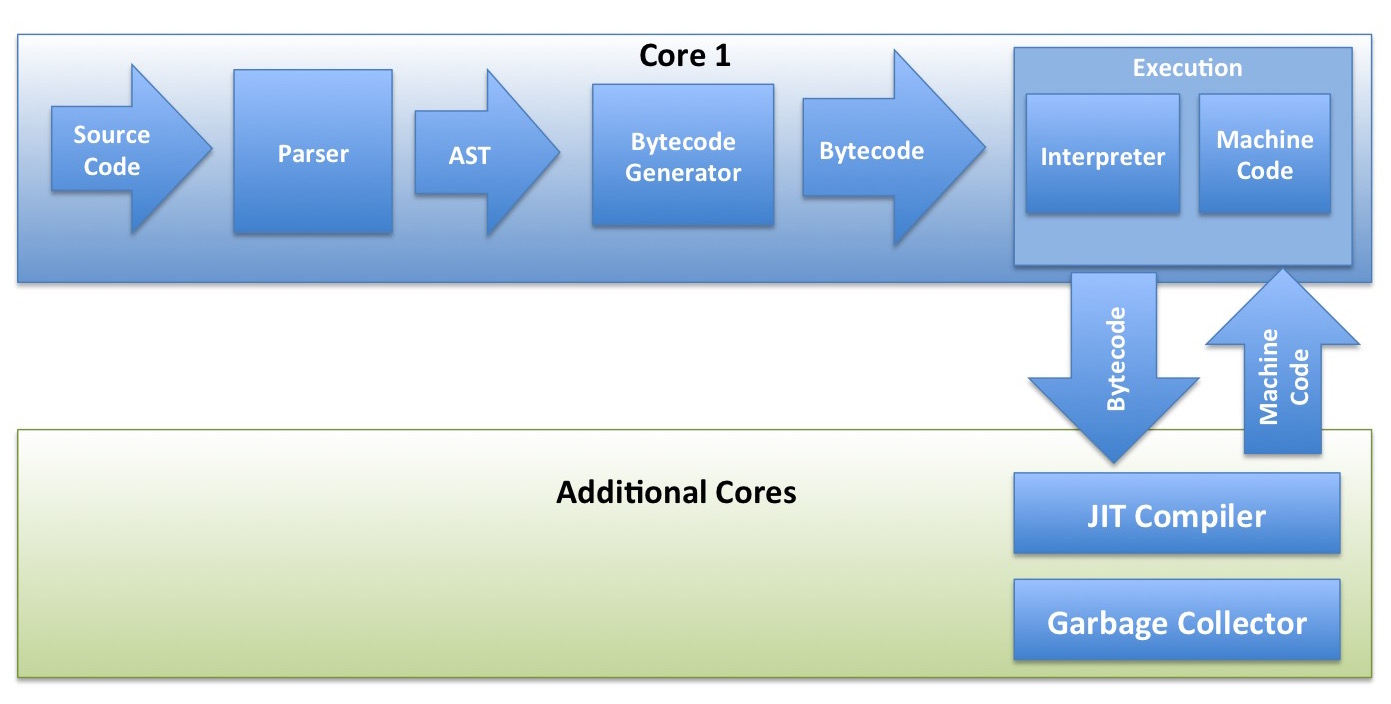
\includegraphics[width=15cm, height=8.25cm]{rhino.jpg}
    \caption[Block Diagram of Rhino Engine]{Block Diagram of Rhino Engine \cite{bib29}.}
    \label{fig:architecture}
\end{figure}

\textbf{Parser}: The input for this module is JavaScript code and the output generated is the Abstract Syntax Tree (AST). The AST is a tree representation of the abstract syntactic structure of a program. For instance, Figure~\ref{fig:ASTcode} represents the AST for the GCD code in Figure~\ref{fig:AST} \cite{bib30}.

\begin{figure}
  \centering
\begin{lstlisting}[language=JavaScript] 
function gcd(a, b)
{
	while (b != 0)
    {
    	if a > b
        	a -= b
        else
        	b -= a
    }
    return a
}
\end{lstlisting}
    \caption[Euclid's GCD algorithm]{Euclid's GCD algorithm.}
    \label{fig:ASTcode}
\end{figure}

\begin{figure}
  \centering
      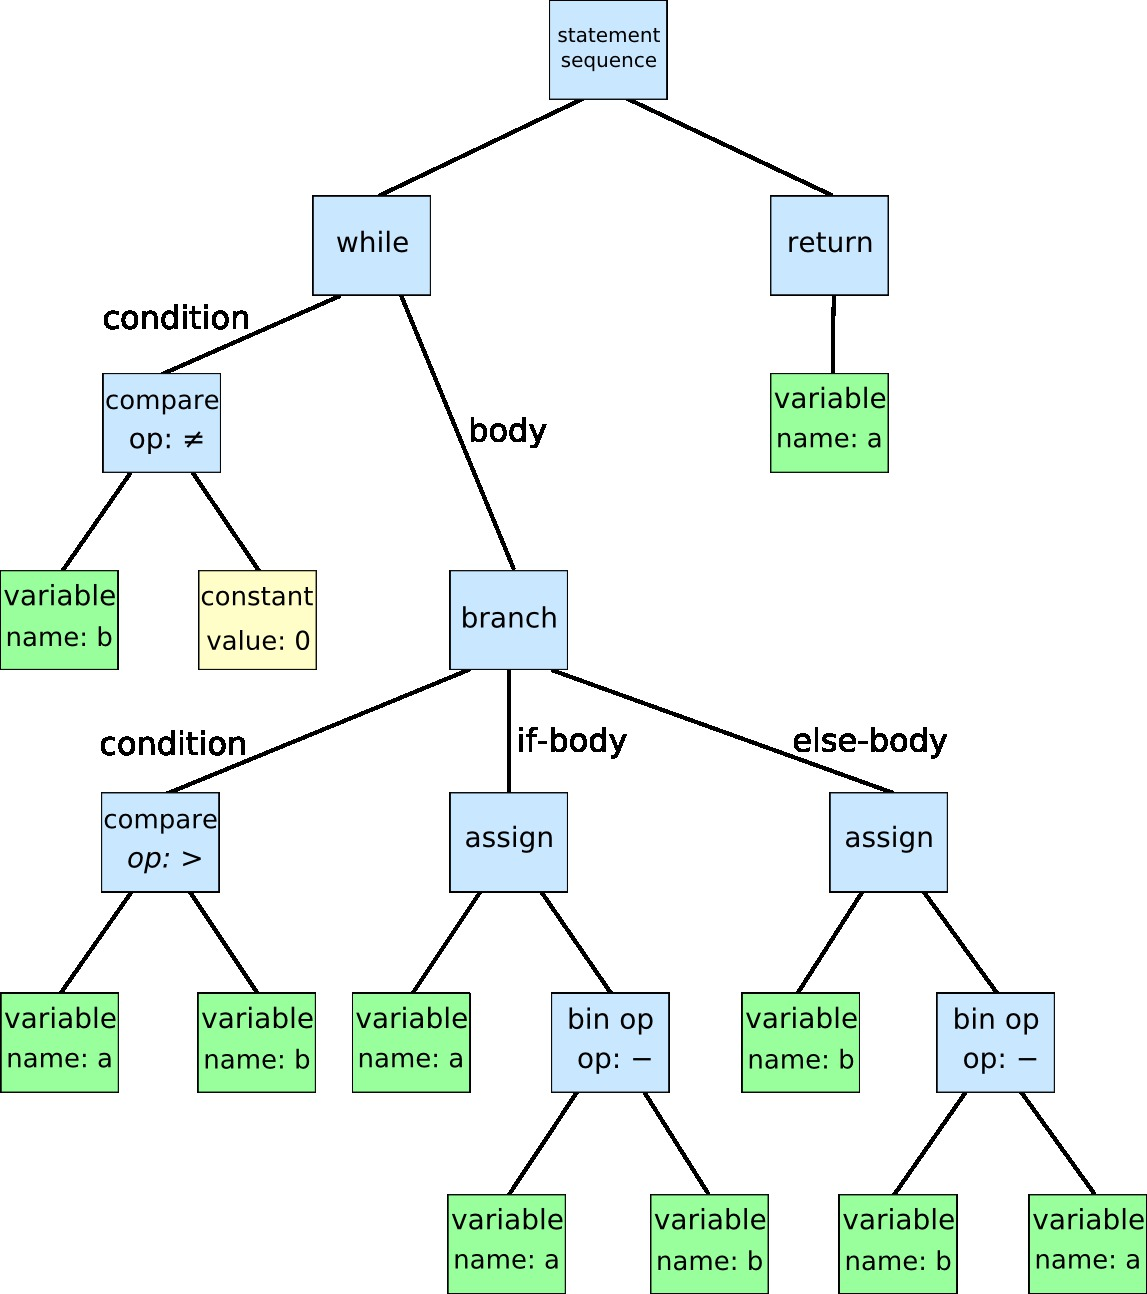
\includegraphics[width=11cm, height=12cm]{AST.jpg}
    \caption[Abstract Syntax Tree]{Abstract Syntax Tree for the GCD code in Figure~\ref{fig:ASTcode} \cite{bib30}.}
    \label{fig:AST}
\end{figure}
The non-leaf nodes in the AST specify the operations to be performed, for instance, equal, comparison, arithmetic operation and so on. The leaf nodes in AST specify operands in the source code, for instance, a and b variables \cite{bib4}. 

\textbf{Byte-Code Generator}: The AST output generated from the parser acts as input to the Byte-Code Generator which then converts the tree into byte code. During the conversion process, the Byte-Code generator picks each code block in the tree and translates it into bytecode. For instance, the byte code for the instruction $c = a - b$ is shown in Figure~\ref{fig:samplebytecode} \cite{bib4}.

\begin{figure}
  \centering
\begin{lstlisting}
iload_1
iload_2
isub 3
istore_3
\end{lstlisting}
    \caption[Sample byte code]{Sample byte code for the instruction $c = a - b$ \cite{bib4}.}
    \label{fig:samplebytecode}
\end{figure}

The bytecode in Figure can be interpreted as - 
\begin{enumerate}
\item Load the values that are stored at offset 1 and offset 2 into registers
\item Subtract these loaded values 
\item Store the result at offset 3.
\end{enumerate}


\textbf{Interpreter}: The input for the interpreter is the byte code output of the Byte-Code Generator. The byte code is then converted into machine level code using the Just-in-time (JIT) compiler. During runtime, this generated machine code gets executed. When the byte code in Figure~\ref{fig:samplebytecode} is given as input to the Interpreter, it generates the machine code as shown in Figure~\ref{fig:samplemachinecode}. 
\begin{figure}
  \centering
\begin{lstlisting}[language=myasm] 
MOV EAX 0xFF20
MOV EBX 0xFF24
SUB EAX EBX
MOV ECX EAX
\end{lstlisting}
    \caption[Sample Machine Code]{Sample Machine Code generated for the byte code in Figure~\ref{fig:samplebytecode} \cite{bib4}.}
    \label{fig:samplemachinecode}
\end{figure}
\subsection{Modification}
For this research, we need the opcodes of JavaScript code, so we used the version of Rhino that was modified by the author of \cite{bib4}.
 
Below changes were made in the modified version \cite{bib4}:

\begin{enumerate}
\item The page load time is directly proportional to compiling time of JavaScript, so Rhino was optimized to convert only small part of JavaScript files. Because of this optimization, the original statistics of the JavaScript code that will be used as part of analysis will get affected. In order to solve this problem the engine was modified to compile JavaScript of any length.
\item Different optimization techniques were used to optimize class files for speed execution. As these optimization techniques also affect the statistics of JavaScript code, they were disabled.
\item Generally opcodes are generated by decompiling the class files. This method consumes a lot of time as this process require the generation of class file and again decompilation of these class files. As the class files generated are of no use, the opcodes are extracted from the code during compilation itself. By following this approach, the time used for decompilation of class files is saved.
\item As the opcodes are extracted before the class file is created, this modification also solved the problem associated with class files optimization.
\item The opcodes are tapped and redirected to the standard output. Thus all the opcodes are printed on the screen. This output can also be saved in a file using the unix redirect operator (>).
\end{enumerate}
 
The below command is used to run the Rhino engine:
\begin{lstlisting}[frame=none,numbers=none,language=JavaScript] 
java -cp <path_to_rhino_js.jar> org.mozilla.javascript.tools.jsc.Main <JavaScript_File_Path>
\end{lstlisting} 
Figures~\ref{fig:codecomprhino} and ~\ref{fig:codecompmodifiedrhino} are the screenshots of compiling JavaScript code with the original version and the modified version of Rhino respectively. 

\begin{figure}
  \centering
      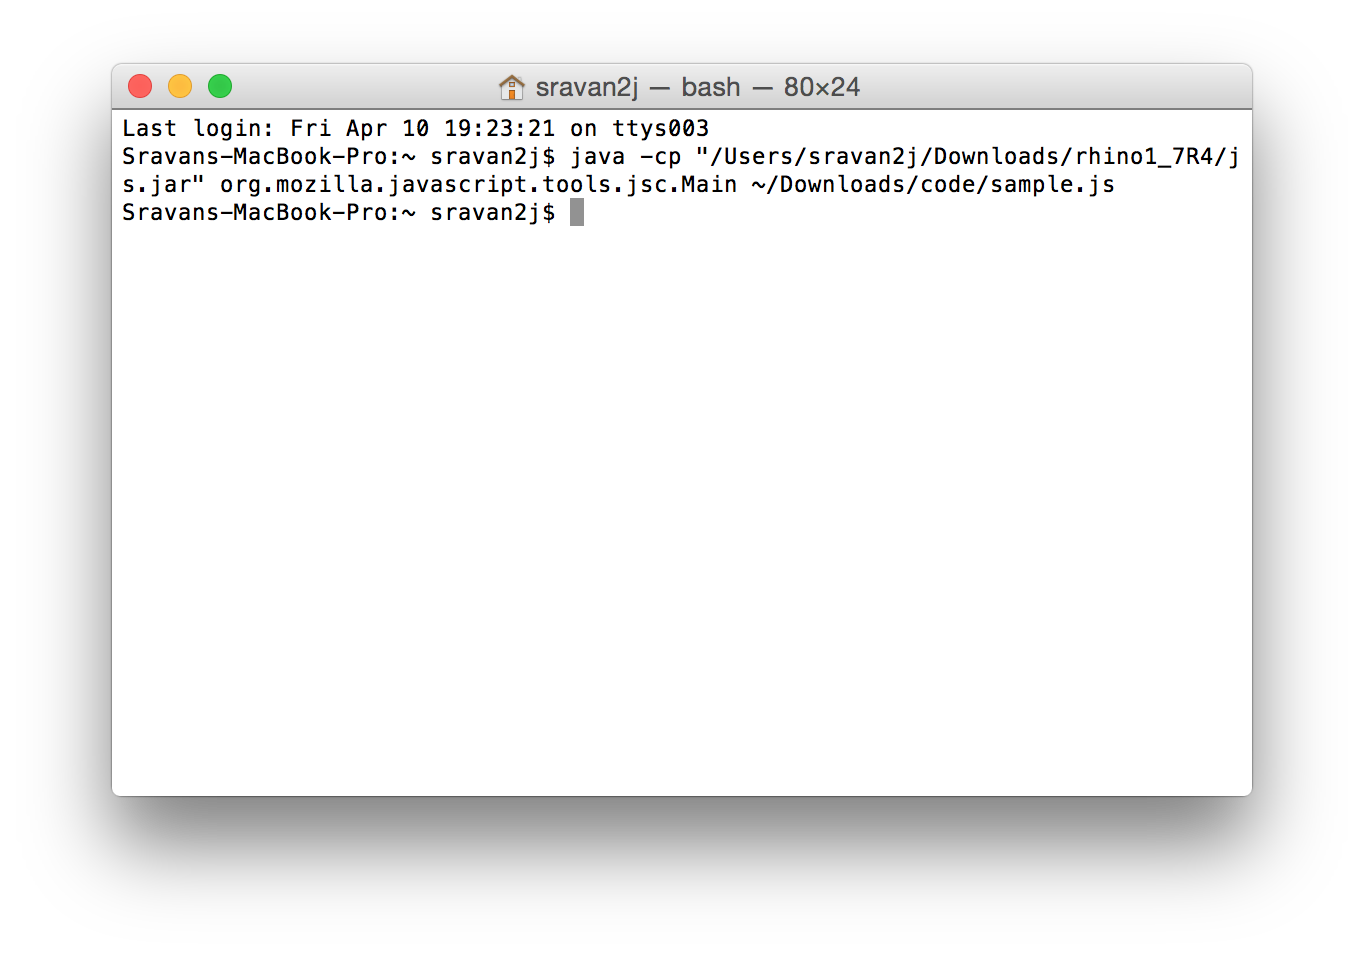
\includegraphics[width=17cm, height=11.95cm]{rhino_screenshot1.png}
    \caption[JavaScript compilation with Rhino]{JavaScript compilation with Rhino.}
    \label{fig:codecomprhino}
\end{figure}

\begin{figure}
  \centering
      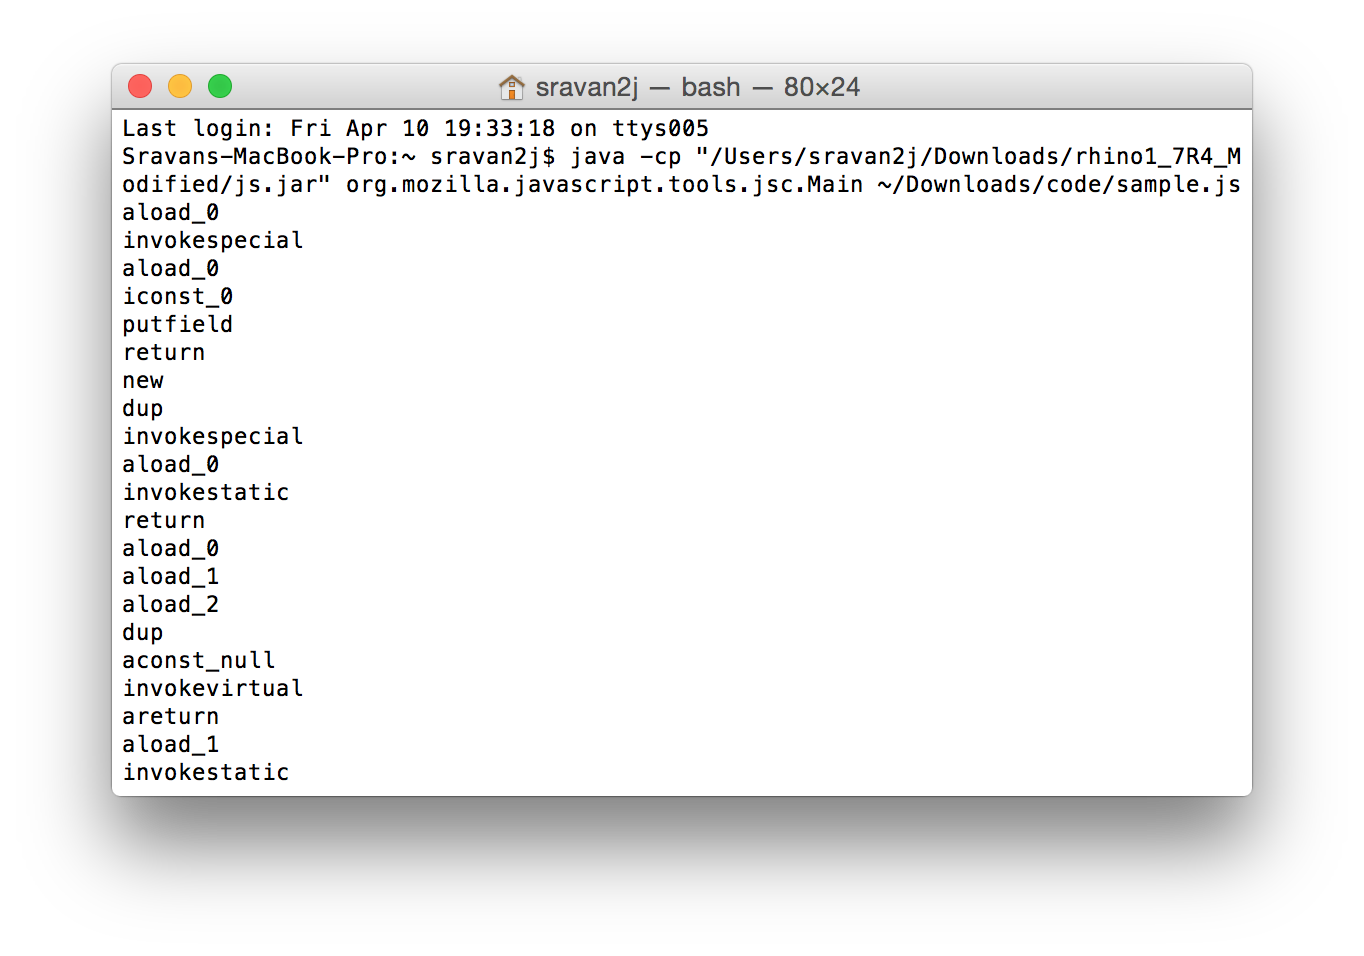
\includegraphics[width=17cm, height=11.95cm]{rhino_screenshot2.png}
    \caption[JavaScript compilation with modified version of Rhino]{JavaScript compilation with modified version of Rhino.}
    \label{fig:codecompmodifiedrhino}
\end{figure}